\begin{abstract}
In this paper, we introduce a general approach to diagnosing
program errors detected by type systems or other program analyses.
This approach works on any analysis that can be described as a
constraint system, in which a detected error corresponds to one or
more unsatisfiable constraints.  Both satisfiable and unsatisfiable
paths through the constraint system are analyzed, to identify the
program expressions most likely to be the cause of the unsatisfiable
constraints. The likelihood of different error explanations is
evaluated under the assumption that the programmer's code is mostly
correct, so the simplest error explanations are chosen, according to
maximum a posteriori principles. For analyses that depend on
programmer-stated assumptions about the environment, the error
diagnosis also identifies likely missing assumptions.  The new error
diagnosis approach has been implemented for two very different program
analyses: type inference in OCaml and information flow checking in
Jif. The effectiveness of the approach is evaluated using a corpus of
previously collected programs containing errors. The results show that
the technique identifies the location of program errors significantly
more accurately than in the original compilers, and also identifies
missing assumptions effectively.

\end{abstract}

\section{Introduction}

Over the past couple of decades, many sophisticated type systems and,
more generally, program analyses have been developed, allowing
complex, important properties of software to be verified. Advances in
type inference, dataflow analysis, and constraint solving have made
programming with such verification more practical, by lowering the
annotation burden and making verification time more acceptable.  Use
of these techniques has become more common, but expressive type
systems are still infrequently used.

We posit that a key barrier to adoption of these sophisticated
analyses is the difficulty of debugging programs when the analysis
reports an error. Because deep, non-local software properties are
being checked, the analysis may detect an inconsistency in a part of
the program that is far from the actual error. Reporting on the
inconsistency at the point of detection can result in a misleading
error message. Determining where the true error lies based on this
error message can require excessive effort from the programmer, and an
unreasonably high degree of understanding of how the analysis works
in order to interpret the error report.

We are motivated to study this problem based on experience with two
programming languages with a reputation for difficult-to-interpret
error messages: ML, whose unification-based type inference algorithm
sometimes generates complex, even misleading error
messages~\cite{wand-errorfinding}, and Jif~\cite{jif}, a version of
Java that statically analyzes the security of information flow within
programs but whose errors also confuse programmers~\cite{king:fse}.
Prior work has explored a variety of methods for improving the errors
reported by each of these languages. However, these methods are often
specialized to the respective languages.

In this work we take a more generic approach to diagnosing the errors
generated by program analyses.  To make the approach generic, we
observe that most program analyses, type inference algorithms, and
type systems can be phrased as constraint-solving problems in which a
system of constraints over variables is to be solved to find values
for the variables.  A system of constraints can be generated from
these various analyses and solved in a generic way by a constraint
solver. For example, in the case of ML type inference, variables
stand for types, and constraints are equalities between different
type expressions mentioning these variables. When the constraint
system is unsatisfiable, the constraint solver at some point
determines there is no way to satisfy some particular constraint. The
question is then how to report this failure, indicating a program
error, to the user. Current practice involves mapping the constraint
back to the program point that generated it, and reporting a
corresponding message. Unfortunately, the actual error in the program
text may be located far from the code that generated the failed
constraint, causing misleading error messages.

Our insight is that when the constraint system is unsatisfiable, a
more holistic approach should be taken to deciding where the program
error is likely to be found. Rather than just looking at the failed
constraint in isolation, the structure of the constraint system as
a whole should be considered. Both satisfiable and unsatisfiable
paths through the constraint system may help identify
the error location.  An expression that is involved
in many unsatisfiable paths is more likely to be erroneous;
an expression that lies on many satisfiable paths is more likely
correct. This approach to identifying errors can be
justified on maximum a posteriori principles, under the assumption
that programmers write code that is mostly correct.

In many languages, the satisfiability of constraint systems may depend
on environmental assumptions (or hypotheses). The conceptual framework
for identifying likely errors can also be applied to identifying likely
missing hypotheses. Again, programmers are not likely to have omitted
many hypotheses, so a small set of hypotheses that makes the constraint
satisfiable is more likely to be correct than a larger set or a large
set of erroneous expressions.
%Recent work on abductive inference~\cite{dillig:pldi12} has studied
%inferring missing hypotheses but has 

\paragraph{Contributions}

This paper makes the following contributions:

\begin{enumerate}
\item
A general constraint language that can model a broad
range of program analyses. It can encode both ML type
inference and Jif information flow analysis
(Section~\ref{sec:language}).

\item
A general algorithm for identifying likely program errors,
based on an analysis of the constraint system corresponding
to the program. This algorithm proposes both program expressions
that are likely to be errors, based on maximum a posteriori
principles, and also hypotheses that the programmer is
deemed likely to have omitted. Importantly,
little language-specific tuning is needed to generate good results.
(Sections~\ref{sec:graph}, \ref{sec:ranking}.)

\item
An evaluation of this new error diagnosis algorithm on two
different sets of programs, including a large set of programs
collected from students using OCaml to do
programming assignments~\cite{lerner:pldi07}
(Section~\ref{sec:evaluation}.)

\end{enumerate}

\section{Program analyses and constraint solving}

%Many program analyses can be modeled as constraint solving problems. In this
%section, we use two apparently different kinds of analyses, information-flow
%control and ML-like language type inference, to motivate why error diagnostic
%is difficult and illustrate the main approach of our work.

\ACM{It would be nice to have a couple of examples here for OCaml and
for Jif where the compiler gets it completely wrong and is misleading,
and that we can use later on to show how the approach is very
effective.}

\paragraph{ML type inference}

The power of type inference is that programmers need not
explicitly write all types. When type inference fails, however,
this power has the downside of possibly confusing error messages.
For example, the following code was written by a student
programmer attempting to solve a programming
assignment~\cite{lerner:pldi07}. (It has been simplified slightly
for clarity.)

% file: stu01, hw1 20060303-20:59:18
\lstset{numbers=left, xleftmargin=15pt, framexleftmargin=15pt}
\begin{lstlisting}
type 'a lst = Null | Cons of 'a * 'a lst

let rec append lst =
  match lst with
    Null -> ()
  | Cons(x,rest) -> Cons(x, append rest lst)
\end{lstlisting}

For this example, the OCaml compiler blames the expression
$\cod{Cons(x,\ append\ rest\ lst)}$ at line 4. But
according to the user's fix, the real error is the expression
$\cod{()}$ at line 3.

To understand why "Cons(x, append rest lst)" is blamed, it
is easier to think of type inference as constraint solving: to find types
that satisfy some constraints induced by program expressions.

For instance, expression $\cod()$, with type "unit", must have the
same type as "Cons(x, append rest lst)" because they are both
returned by function "append". Hence, type inference fails since these two expressions have different types---they cannot
be unified.

Although it might seem arbitrary to blame one of these two expressions to
blame, there is a reason why "()" is _more likely_ to be wrong.
Notice that the return type of function "append" is also
used as the second parameter in constructor "Cons".  By the
definition in line 1, it has the same type as "Cons(x, append rest lst)".
Therefore, assuming that the programmer is less likely to make many
mistakes, "()" appears more likely to be wrong.

The approach of inferring likely wrong expressions is more powerful in
the following student program, for which the location reported by the
OCaml compiler is confusing.

%file: stu01, hw2-logo 20060319-20:22:42
\begin{lstlisting}
let p1 (lst : move list) : (float*float) list = 
  let p2 lst x y dir : 
    move list * $\shadow{float}$ * float * float = 
  match lst with
  | [] -> raise EmptyMoveList
  | Home::tl -> (tl, $\shadow{2}$, 0.0, 0.0)
  |  ... (* more statements *)... 
  in
  let rec loop lst $\shadow{x}$ y dir acc =
    match p2 lst $\shadow{x}$ y dir with
      (List,$\shadow{nX}$,nY,Dir) -> 
        if($\shadow{x}$ <> $\shadow{nX}$) then print_string "no match";
        failwith "implement";
  in 
  List.rev (loop lst $\shadow{0.0}$ 0.0 0.0 [(0.0,0.0)])
\end{lstlisting}

For this example, OCaml reports that the whole match expression (lines
4--7) is wrong. This error message is misleading because the programmer's
fix shows that the real error is that the "2" at line 6 should be "2.0".
%Moreover, the shadowed variable name $\cod{lst}$ (we preserved them in
%this example) makes finding the error more challenging.

The error location can be inferred by the same kind of reasoning as
above: we notice that all highlighted
expressions must have the same type. The intuition is that
the type expression "2" is inconsistent with that of the several
other highlighted expressions that must have the same type;
excluding "2", the type constraints are satisfiable along the path
$\cod{0.0=x_{9}=x_{10}=x_{12}=nX_{12}=nX_{11}=float}$ (where the
subscript identifies the line number).

Prior work has explored the idea of tracing and reporting everything
along paths related to a type inference
failure~\cite{wand-errorfinding,choppella95, haack:slicing,
tip:slicing}. Our goal is to be more useful, by identifying the
precise point along the path where the error occurs. However,
constructing such paths is an intermediate step in our approach.
%Clearly, such result requires much more efforts to
%identify the error compared with our precise location report (though
%our approach also generates such information in an intermediate step).

% % stu02, hw2-logo 20060322-14:52:42
% \begin{lstlisting}
% let result = (2.0*3.1416)
% \end{lstlisting}
% 
% This is a simple one, OCaml blames 2.0, but the error is that (*.)
% should be used.
% 
% % file: stu03, hw2-imp 20060323-23:05:28
% \begin{lstlisting}
% let lookup_var h str = 
%   match lookup_raw h str with
%     0 -> 0
%   | Var(_,i) -> i
%   | Heap(_) -> 0
% \end{lstlisting}
% 
% This is a simple one, OCaml blames $\cod{Var(_,i)}$, but the error is that 0
% should be Nil.
%

\paragraph{Jif label checking}

Jif~\cite{jif} is a Java extension that statically analyzes the
security of information flow within programs. 

Jif can generate confusing error messages~\cite{king:fse} that result
from the constraint solving process it uses to infer security labels.
In many cases, the error results from a failure to write down
assumptions about trust relationships in the program.

For instance, an assignment from a memory location labeled with a
patient's security label to another location with a doctor's label
may fail to label-check because the hypothesis that doctor acts for
patient---meaning that the security model allows the flow from patient
to doctor---is missing. 

In this paper, we also propose a general way to infer likely
missing hypotheses.

\section{Constraint language}
\label{sec:language}

A key component of our approach is a general core constraint language
that can be used to capture a large class of program analyses.
In this constraint language, constraints are inequations using an
operator ≤ corresponding
to a flow of information through a program. The constraint language
also supports constructors and destructors corresponding to
computation.
%How information flow control and ML-like type
%inference can be expressed by this language is also discussed. 

\subsection{Syntax}

The syntax of the constraint language is formalized in
Figure~\ref{figure:lang:syntax}.

\begin{figure}
\hfil
\begin{minipage}{2in}
\begin{align*}
G &::= G_1 \land G_2 \bnf A \\
A &::= C_1 \proves C_2 \\
C &::= I_1 \land ... \land I_n~~^{n≥0} \\
I &::= E_1 ≤ E_2 \\
E &::= x \bnf c(E_1,\dots,E_{\arity{c}}) \bnf \invcabs{c}{i}(E) \\
  & \bnf E_1 \join E_2 \
\bnf E_1 \meet E_2 \bnf \bot \bnf \top
\end{align*}
\end{minipage}
\hfil
\caption{Syntax of constraints}
\label{figure:lang:syntax}
\end{figure}

The top-level goal $G$ to be solved is a conjunction of assertions $A$. An
assertion has the form of $C_1 \proves C_2$, where constraint $C_1$ is the
hypothesis and constraint $C_2$ is a conclusion to be satisfied.
 
Constraint $C$, either serving as the hypothesis or the conclusion, is a
possibly empty conjunction of inequations $I$ over elements from $E$,
based on some ordering $≤$. We denote an empty conjunction as ∅,
and abbreviate $∅ \proves C_2$ as $\proves C_2$.

An element $E$ may be a variable $x\in\varset$ whose value is to be
solved for, a constructor application $c$ or the $i$-th projection
($i$-th component) of a constructor application, represented by
$\invcabs{c}{i}(E)$. The arity of constructor $c$ is represented
as $a(c)$. Constants $c$ are nullary constructors, with arity 0.
For example, if modeling ML type inference, we can
represent the type "int->bool" as a constructor application
$\cons{fn}{\atom{int}, \atom{bool}}$, where $\atom{int}$
and $\atom{bool}$ are constants.
Its first projection $\invc{fn}{1}
(\cons{fn}{\atom{int}, \atom{bool}})$ is equal to $\atom{int}$.
%
Elements can also be the join ($\join$) or meet ($\meet$) of elements.
The bottom and top of the element ordering are 
$\bot$ and $\top$.
%When join and meet are
%used, we assume for all $e_1, e_2 \in E, e_1 \join e_2 \in E \land e_1
%\meet e_2 \in E$ to make the constraints well-formed. In another word,
%the elements form a lattice.

\ACM{What are the requirements for a well-formed goal? Presumably
constructors and projections have to be used with the correct arities.
Is there some additional type restriction?  I assume the same variable
can appear in multiple assertions, but this is not clear from the
presentation.}

\subsection{Interpretation of constraints}

The ordering $\leq$ is treated abstractly by our diagnosis algorithm,
but it must define a lattice. The operators $\join$ (join) and $\meet$
(meet) produce the least upper bound and greatest lower bound
of their operands, respectively.
%
The elements $\bot$ and $\top$ are respectively the least and greatest
element with respect to $\leq$.

We further assume that the partial ordering on constructor applications
is determined by the polarities of that constructor's arguments.
For each argument, the ordering of constructor applications is either
covariant with respect to that argument (denoted by "+"),
contravariant with respect
to that argument ("-"), or invariant with respect to that argument
("0").
%That is, $\forall c\in \conset, c(E_1, \dots, E_{a(c)})\leq c(E_1',
%\dots, E_{a(c)}') \Iff E_1\leq E_1' \land \dots, E_{a(c)}\leq
%E_{a(c)}'$.

With these abstract definitions, the _validity_ of variable-free constraints can be defined
in a natural way. A variable-free goal $G$ is valid if all assertions it contains are valid.
An assertion $C_1 \proves C_2$ is valid if
the partial orderings in $C_2$ can be inferred from $C_1$, using just
the lattice properties of the relation ≤ and the polarities of the
various constructor arguments.
%Thus, validity of an assertion does not
%depend on how variables are instantiated.

\paragraph{Example}

Let $c_1, c_2, c_3$ be three constants. Then $c_1 \leq c_2 \land c_2 \leq c_3
\proves c_1 \leq c_3$ is valid by the transitivity of $\leq$. Assertion
$\proves c_1 \leq c_1 \join c_2$ is valid by the definition of join. But
assertion $\proves c_1\leq c_2$ is invalid since the
conclusion cannot be inferred from the empty assumption.

\subsection{Satisfiability}

Validity as defined so far works for constraints without variables.
When constraints mention variables, we want to know whether there
exists a valuation of all variables such that the goal after value
substitution is valid or not. This is formalized as _satisfiability_
of constraints.

Satisfiability depends on the _ground terms_ $\termset$ 
that a variable can map into. We define $\termset$ as the
greatest fixed point of the following rules:

\begin{itemize}
\item All constants are in $\termset$.

\item $c(t_1, \dots, t_{\arity{c}})\in \termset$ if 
$\forall_ {i∈\{1,\dots,a(c)\}}~t_i \in \termset$ and $c\in C$.
\end{itemize}

\noindent
Notice that ground terms may be infinite. This feature is essential for
modeling recursive types.

% All terms form a Herbrand universe under $\join$ and $\meet$.

A valuation $\valuation: \varset→\termset$ is a function from
variables to terms. A goal is _satisfiable_ when there exists a
valuation $\valuation$ such that the goal is valid after substitution using
\valuation.

\paragraph{Example}

Let $x\in \varset$, $c_1, c_2, c_3\in \termset$. Then $\proves x \leq c_1$ is
trivially satisfiable by the valuation $\valuation(x)=c_1$ or
$\valuation(x)=\bot$. However, $\proves x \leq c_1 \land c_2 \leq x$ is
unsatisfiable since otherwise, $c_2 \leq c_1$ by the transitivity of
$\leq$, yet this ordering on $c_1, c_2$ cannot be inferred.

Infinite terms are needed to solve some constraints. For instance,
$\proves x \leq \cons{\textit{c}}{\atom{zero}, x}$, where $\atom{zero}
\in \conset \land a(\atom{zero})=1$ and $x\in \varset$ is satisfiable
by replacing $x$ with $c(\atom{zero}, c(\atom{zero}, \dots))$.
\ACM{This seems broken. a(zero) = 0, right? and a(c) = 2?}
\ACM{It would be nice to understand why we need infinite terms.
In particular, might the infinite terms be incorrect solutions
to some constraint systems?}


\subsection{Errors and explanations}

Recall that the goal of this work is to diagnose the cause of errors.
Therefore we are interested not just in the satisfiability of a
set of assertions, but also in where to place the blame when
a goal is unsatisfiable. In our approach,
an _explanation_ consists of a subset of elements from the constraint
system, constraints from the constraint system, and possibly some
missing hypotheses. The goal is to find the most plausible
explanation for the failure of satisfiability. 

Under the assumption that programmers write mostly correct code,
explanations are more plausible when they involve fewer and more
likely programmer errors. To keep this diagnostic method as general as
possible, we avoid building in domain-specific knowledge about which
errors programmers tend to make.  However, the framework does
accommodate adding such knowledge in a straightforward way.

\ACM{What happened to our story about mixed explanations that
consist of constraints + hypotheses? The distinction here between
erroneous elements and erroneous constraints is a bit confusing.}

\paragraph{Incorrect constraints}

One cause of unsatisfiability is the existence of some constraints
in the goal's conclusions. We say that a set of constraints
$\mathcal{C}$ is _inconsistent_ if removing those constraints from
goal conclusions make an unsatisfiable goal satisfiable.

\paragraph{Example}

Consider the unsatisfiable goal $\proves x \leq c_1 \land c_2 \leq x$
again. Another possible cause of the unsatisfiability may be that one
of the constraints $x \leq c_1$ and $c_2 \leq x$ is wrong. 

\paragraph{Missing hypotheses}

A second cause of unsatisfiability is the absence of constraints in
the hypothesis. Such error corresponds to the failure to write down
assumptions.

\paragraph{Example}
Consider the unsatisfiable goal $\proves x \leq c_1 \land c_2 \leq x$.
One possible cause of the unsatisfiability may be the omission of a
hypothesis $c_2\leq c_1$.
\ACM{I flipped this hypothesis around, hopefully correctly...}

\if 0
\paragraph{Relation with set constraints}

Although the core constraint language is similar in spirit to set
constraints~\cite{aiken-setconstraint}, there are several notable
differences:

\begin{enumerate}

\item Most importantly, this constraint language models hypotheses,
enabling the modeling of some existing program analyses, such as the
``where'' clause in Jif and the subtype constraints used in Java
generics.

\item We exclude the negation of elements in our model since it is not
essential in modeling many program analyses. Also, previous work
showed that the complexity of solving the full set of set constraints
is NP to NEXPTIME~\cite{aiken-complexity}. We believe that the
proposed constraint language is expressive enough for most program
analyses of interest.

\end{enumerate}
\fi

\subsection{Expressiveness}

% Due to the similarity between our core constraint language and set
% constraint, the applications modeled by the later without negations
% are automatically expressed by our model. Such examples includes type
% inference with sum type and product type and closure analysis.

To show how the constraint language can model a variety of different
program analyses, we discuss how both information-flow control and ML
type inference with polymorphism can be expressed by our constraint
language.

\subsubsection{Information-flow control}

% The security labels can be modeled by the constants in our constraint language.
% $\leq$ is interpreted as ``less restrictive'' in this problem domain. The join
% and meet operations in constraints are consistent with that in the lattice.
% $\bot$ is the most public label, while $\top$ corresponds to the most
% restrictive one. 

% In this part, we focus on a sophisticated information-flow control model, the
% DLM model~\cite{ml-ifc-97}, due to the following challenging features. Of
% course, models with less intricacy can also be described by our core constraint
% language.
% 
% \begin{enumerate}
% \item The label model is more complicated than traditional multilevel security
% system.
% 
% \item DLM introduces an implicit form of parametric polymorphism, called _label
% polymorphism_, to express procedures that are parametric with respect to the
% security labels of their arguments.
% 
% \item DLM allows assertions on labels to enable the combination of a static
% program analysis provably enforces security under some assumptions, while the
% validity of the assumptions are enforced at runtime. 
% \end{enumerate}
% 

In information-flow control systems, information is tagged with security
labels, such as ``unclassified'' or ``top secret''. Such 
security labels naturally form a lattice~\cite{denning-lattice},
and the goal of such systems is to ensure that all information flows
upward in the lattice.

To demonstrate the expressiveness of our core constraint language, we
show that it can express the information flow checking in 
the Jif language~\cite{jif}.
%Of course, less intricate models can also be described by our core
%constraint language.

\paragraph{Label inference and checking}

Jif~\cite{jif} is a version of Java that statically analyzes the security of
information flow within programs based on the DLM model~\cite{ml-ifc-97}. In
this language, types are annotated with security labels.

Information flow is checked by the Jif compiler using constraint
solving. For instance, given an assignment $x := y$, the compiler
generates a constraint $L(y)\leq L(x)$, meaning that the
label of $x$ must be more restrictive than that of $y$.

Moreover, the programmer can omit some security labels and let the
compiler generate them when possible. For instance, when the label of
$x$ is not specified, assignment $x := y$ generates a constraint
$L(y)\leq \alpha$, where $\alpha$ is a label variable to be inferred.
Hence, Jif constraints are broadly similar in structure
to our general constraint language.

However, some features of Jif are challenging to model.  In fact, to
the best of our knowledge, our constraint language is the first
general constraint language expressive enough to model these features.

\paragraph{Label model}

The basic building block of the DLM model is a set of _principals_
representing users and other authority entities. Examples of
principals could be patient A, patient B, doctor A and so on.
Principals can be expressed by constants.

Labels form a lattice, but principals themselves are also structured
as a lattice with respect to a relation _actsfor_.  The proposition
$\cons{actsfor}{A,B}$ means that $A$ is at least as privileged than
$B$.
% 
For instance, if doctor A _actsfor_ patient A, then doctor A is
allowed to read all information that patient A can read. However, such
relation does not grant doctor A to read any information patient B can
read, unless doctor A _actsfor_ patient B too. The _actsfor_ relation
can be expressed by the partial ordering $\leq$.

Security policies on information are expressed as _labels_ that
mention these principals.
A label $L$ contains a set of principals called the
_owners_.  For each owner $O$, the label also contains a set of
principals called the _readers_. Readers are the principals to whom
owner $O$ is willing to release the information. 

For instance, a label $\lab{o_1:r_1,r_2;\ o_2:r_2,r_3}$ can be read
as: principal $o_1$ allows principals $r_1$ \emph{or} $r_2$ to read
the tagged information, \emph{and} principal $o_2$ allows principals
$r_2$ \emph{or} $r_3$ to read.  Hence effectively, only the principals
in the _effective reader set_, the intersection of the readers of all
owners, may read the information.
\newcommand\readers{\mathit{readers}}

In the presence of the _actsfor_ relation $\leq$, the effective reader set is
defined as follows:
\[\readers(p, o→r) ≜ \{q  \mid \text{if}\ p \leq o\ \text{then} (o \leq q\
\text{or}\ r \leq q)\}\]

Based on this definition, the ``no more restrictive than'' relation
$\sqsubseteq$ on confidentiality policies is formalized as:
\[ c \sqsubseteq d \Iff \forall p.~\readers(p, c) ⊇ \readers(p, d) \]

Because of this definition, a confidentiality policy in the DLM
model can be treated as a covariant constructor on principals.
Integrity policies are dual to confidentiality policies, so they
can be treated as contravariant constructor on principals.

\ACM{Not clear this theorem is sufficiently interesting to spell
out in detail. Also, presumably there is an integrity policy
property to be stated?}

\iftr
\begin{Theorem}
A confidentiality policy in the DLM model is a covariant constructor
on principals.
\end{Theorem}

\begin{proof}
It is sufficient to show that $a→b \sqsubseteq c→d \Iff a\leq c \land
b\leq d$.

$\Longrightarrow$: by definition, $readers(a, a→b) ⊇ readers(a, c→d)$.
If $a\not\leq c$, then the second part is the entire principal space.
This is a contradiction since $\bot\not\in readers(a, a→b)$. Given $a\leq c$, $d
\in readers(a, c→d)$. So $d \in readers(a, a→b)$. That is, $a\leq d$
or $b\leq d$. In either case, we have $b\leq d$ by noticing that $a$
is an implicit reader of $a→b$, or, $b=a\meet \dots\leq a$.

$\Longleftarrow$: consider any principal $p$. If $p\not\leq a$,
$readers(p, a→b)$ is the entire principal space, hence result is
trivial. Otherwise, $p\leq a \leq c$. Hence, sufficient to show that
$\{q \mid a\leq q\ \text{or}\ b\leq q\} ⊇ \{q \mid c\leq q\ \text{or}\ d\leq
q\}$ which is obvious from assumptions.

\end{proof}
\fi

\paragraph{Label polymorphism}

Polymorphism makes it possible to write reusable code that is not tied
to any specific security policy. One common form of polymorphism is
over the labels of method parameters. 

For instance, consider a function "foo"
with the signature "int foo(bool\lab{Alice→Alice} b)".
Instead of requiring the parameter "b" to have exactly the label
"\{Alice→Alice\}", the label actually serves as an upper bound on the
real parameter.

The introduction of hypotheses in our constraint language makes the
modeling of such label polymorphism straightforward. Instead of
requiring the label of "b" to
be "\lab{Alice→Alice}", we add the constraint $c_{\,\texttt{b}} \leq
"\lab{Alice→Alice}"$ to the hypotheses of all constraints generated in the
method body, where $c_{\,\texttt{b}}$ is a constant representing the label of
variable "b".

\paragraph{Method constraints}

Methods in Jif may contain ``where'' clauses, explicitly stating
constraints assumed to hold true during the execution of the method
body. The compiler type-checks the method body under these assumptions
and checks that the assumptions are true at all method call sites. 
Method constraints are easily modeled by hypotheses in our
constraint language.
 
\subsubsection{ML type inference}

ML type inference can also naturally map into constraint solving. Numerous 
efforts have been made in this direction. For instance,
Wand~\cite{wand-typeinference} recast Hindley-Milner type system into equality
constraints. Aiken and Wimmers~\cite{aiken-typeinclusion} extends the
Hindley-Milner type system with inclusion constraints, and models function
types, constructor types, liberal intersection and union types. Haack and Wells
~\cite{haack:slicing} recast Damas’s algorithm T into constraints.

Since most of these constraint languages are similar, we discuss how
the _labeled constraints_ proposed in~\cite{haack:slicing} can be
transformed to our language. We pick this constraint language since it
supports let-polymorphism, and our evaluation extends one
implementation of this approach on OCaml.

For simplicity, we only discuss a subset of ML-like language, syntax shown in
Figure~\ref{figure:mltypes} in this part, though a larger sublanguage
of OCaml can be handled in similar way.

\newcommand\expr{\mathit{e}}
\newcommand\ty{\mathit{t}}
%\newcommand\ty{\mathit{ty}}

In this language subset, expressions can be variables ($x$), integers
($n$), operation on two expressions ($+$), functions $\fn~x→\expr$,
function application ($\expr_0~\expr_1$), or let bindings
($\kwlet x = \expr_1 \kwin \expr_2$). Notice that
let-polymorphism is allowed since the expression in the let binding
may contain free variables.

Haack and Wells~\cite{haack:slicing} show that type-checking the
language of Figure~\ref{figure:mltypes} is equivalent to a set of
type constraints of the form $\ty = \ty'$.

Types $\ty$ in the constraints are defined as follows.
\[\ty ::=\; x \mid \atom{int} \mid \ty \rightarrow \ty\]
\noindent where $x$ is a type variable to be inferred, $\atom{int}$ is the predefined type integer and
$\rightarrow$ is the predefined constructor, function type. Because
the details of the
transformation from typing rules to constraints
are less relevant, see~\cite{haack:slicing} for more details. 

Labeled constraints form a strict subset of our constraint
language:
%($L$ is just the annotation on the constraints)
types $\ty$ are elements, and equality $\ty=\ty'$ is equivalent to
$\ty\leq \ty' \land \ty'\leq \ty$. 

\begin{figure}
\begin{minipage}{2in}
\begin{align*}
\expr ::=  & x \mid n \mid \expr_1 + \expr_2 \mid \fn x → \expr \mid
\expr_0  \expr_1 \mid \kwlet x =
\expr_1  \kwin  \expr_2
\end{align*}
\end{minipage}
\caption{Syntax of a subset of ML}
\label{figure:mltypes}
\end{figure}


% In this setting, types are the elements. Join and
% meet operations are the usual intersection and union types if that is
% well defined.
% $\leq$ is consistent with the subtype relationship between two labels.
% Since the definition is abstract, both syntactic subtyping \DZ{REF}
% and semantic subtyping~\cite{aiken-typeinclusion} fit in this model.
% 

\if 0
The syntax and transformation rules are stated in
Figure~\ref{figure:ml-constraints} (we simplified the rules
in~\cite{haack:slicing} for better presentation).

\begin{figure}
\hfil
\begin{minipage}{2.3in}
\begin{align*}
\expr ::=  & x \mid n \mid \expr  +   \expr \mid \fn  x \rightarrow \expr \\
        & \mid \expr  \expr \mid \kwlet  \val  x = \expr  \kwin 
	\expr  \kwend
\end{align*}

\begin{mathpar}
\inferrule{}{x \Downarrow \configThree{\emptyenv\{x\mapsto \{a_x\}\}}{a}{\{a_x=a\}}} \text{ where $a_x, a$ fresh}
\and
\inferrule{}{n \Downarrow \configThree{\emptyenv}{a}{\{int=a\}}} \text{ where $a$ fresh}
\and
\inferrule{\expr_1 \Downarrow \configThree{\G_1}{ty_1}{C_1} \and \expr_2 \Downarrow \configThree{\G_2}{ty_2}{C_2}}
{\expr_1+\expr_2 \Downarrow \configThree{\G_1\union\Gamma_2}{a}{\{ty_1=int;ty_2=int\}\union C_1\union C_2}} \text{ where $a$ fresh}
\and
\inferrule{\expr \Downarrow \configThree{\G}{ty}{C}}
{\fn\; x \rightarrow \expr \Downarrow \configThree{\G[x\mapsto \{\}]}{a}{\{a_x=ty' \bnf ty'\in S\}\union\{a_x\rightarrow ty = a\}\union C}} \text{ where $a$ fresh}
\and
\inferrule{\expr_1 \Downarrow \configThree{\G}{ty}{C}}
{\fn\; x \rightarrow \expr \Downarrow \configThree{\G[x\mapsto \{\}]}{a}{\{a_x=ty' \bnf ty'\in S\}\union\{a_x\rightarrow ty = a\}\union C}} \text{ where $a$ fresh}

\end{mathpar}
\end{minipage}
\hfil
\caption{Syntax and constraint generating rules}
\label{figure:ml-constraints}
\end{figure}


Type inference is reduced to constraint solving by defining a mapping
of _pre-judgments_to constraints:
\[\trans{\G \proves x:\tau} = x =\tau\]
\[\trans{\G \proves \lambda x.e:\tau} = \exists a_1 a_2.
(def x: a_1 in \trans{e:a_2} \land a_1 \rightarrow a_2 =\tau)\]
\[\trans{\G\proves e_1 e_2 : \tau} = \exists a.(\trans{\G \proves
e_1:a\rightarrow \tau}\land \trans{\G\proves e_2:a})\]

\DZ{We may eliminate the 'exists' by creating fresh variables}

\paragraph{Polymorphic Types}

Our model is also powerful enough to capture polymorphic types.  Jif
has polymorphic labels. Polymorphic types are also important for
ML-like languages.

Polymorphic types can be naturally modeled in our core constraint
language as follows. For a polymorphic type $t$ instance, we create a
new constant $c_t$ and replace all occurrences of $t$ with $c_t$ in
the constraints. This is sufficient since the semantics of a
polymorphic type is that the constraints should be satisfied
regardless of the value of $t$. For instance, $t\leq \top$ where $t$
is a polymorphic type is satisfiable.
\fi

\section{Constraint graph} 
\label{sec:graph}

The core constraint language has a natural graph representation that
enables analyses of the system of constraints. The key insight is that
satisfiability of the constraints corresponds to reachability in the
graph.

%Inferring provable $\leq$ ordering on the constraints is
%translated into context-free-language reachability in the graph (with
%specially rules for joins and meets). Hypothesis of the assertions are
%used to construct a hypothesis graph in the same way, which checks the
%satisfiability of a path in graph.

\subsection{The intuition behind the transformation}

We use a simple example to illustrate the key ideas behind the
transformation to a constraint graph.  This example shows we
identify subsets of unsatisfiable constraints from a _constraint
graph_ generated from constraints.

\paragraph{Example} Consider the following set of constraints.
\begin{align*}
      &\; \proves x \leq \fn (\cod{ty1}, \cod{bool})  ~~\land~~
          \proves \fn (\cod{ty2}, \cod{int}) \leq y \\
\land &\; \cod{ty1} ≤ \cod{ty2} \proves y \leq x
\end{align*}

In this example, we can interpret $\leq$ as the subtyping relation. $\fn$ is
a function type where the first parameter is contravariant and the second
parameter is covariant. The identifiers $\cod{ty1}, \cod{ty2}, \cod{bool},
\cod{int}$ are constants and $x, y$ are type variables to be inferred.

The first assertion claims that $x$ is a subtype of $\fn ("ty1",
"bool")$, with no hypotheses. The second is similar.
The third assertion says that $y$ is a subtype of $x$ if "ty1" is
a subtype of "ty2".

To check if this goal is satisfiable or not, the key idea is to
identify inconsistency in the constraints, by applying the inference
rules associated with the relation $\leq$ and the operators $\join$
and $\meet$ until a conflict is identified. Such
inference is equivalent to finding all reachable node pairs in a
constraint graph where the all labels along the path can be reduced to
a nonterminal according to a context-free grammar.

\paragraph{Constraint graph construction}
To start, the partial order $\leq$ corresponds to a directed edge in
the constraint graph; elements are presented by nodes. However,
non-constant constructors and hypotheses needs more dedicate
transformation.

Consider the element $\fn (\cod{ty1}, \cod{bool})$. We need to capture
the fact that the constructor is decomposable in the graph. The idea is to add
special _constructor edges_ between the constructor and its
components, as illustrated in Figure~\ref{fig:consgraph}(a).

\begin{figure*}
\newcommand\fh{11em}
\begin{center}
\subfigure[Constructor edges]{
    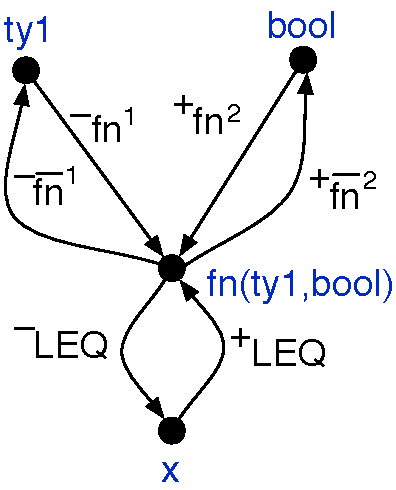
\includegraphics[height=\fh]{graph/onecons}
    \label{fig:consgraph:first}
}
\qquad
%
\subfigure[Constraint graph]{
    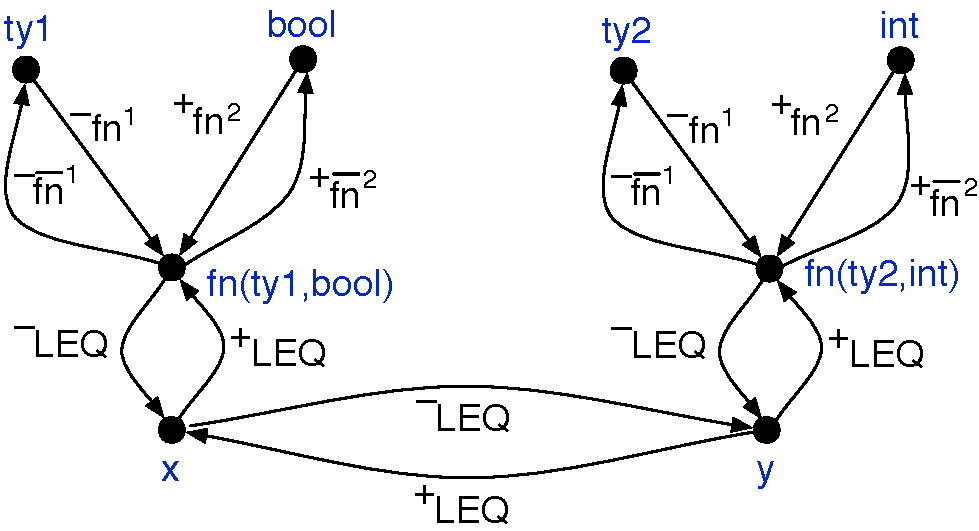
\includegraphics[height=\fh]{graph/consgraph}
    \label{fig:consgraph:second}
}
\qquad
%
\subfigure[Hypothesis graph]{
    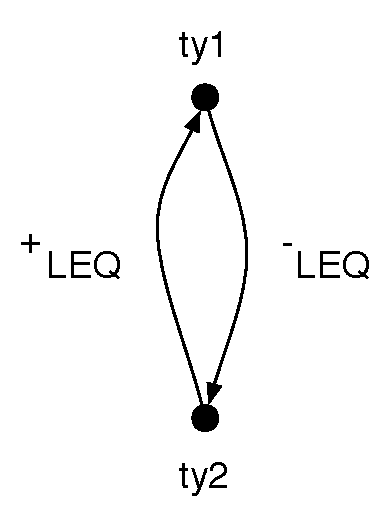
\includegraphics[height=\fh]{graph/hypograph}
    \label{fig:consgraph:third}
}
\end{center}
\caption{Example of a constraint graph}
\label{fig:consgraph}
\end{figure*}

Constructor edges are labeled by the following information: the constructor,
position of the component, and the polarity (covariant, contravariant or
invariant). For instance, the edge labeled $\polarity{+}{\consi{fn}{1}}$
connects the first (covariant) component to the constructor
application.
%
Decomposition edges are also added from the constructor applications
to the components, distinguished by a overline above the constructor
name in the graph.

To enable the flow from potentially contravariant variables, the LEQ edges,
representing $\leq$ relation, are duplicated in the reverse direction with
polarity $-$. For instance, there are two LEQ edges connecting $x$ and
$\fn(\cod{ty1},\cod{bool})$, with different polarity and direction.

Some edges are conditioned on hypotheses, such as the third constraint
$\cod{ty2} \leq \cod{ty1} \proves y \leq x$. For assertions with
hypotheses, we construct the edges as discussed so far, and save the
hypotheses on the edges to be used later.

The transformed graph is shown in Figure~\ref{fig:consgraph:second}. The
systematic way of constructing a constraint graph from constrains is covered in
Section~\ref{sec:consgraph}.

\paragraph{Inferring $\leq$ ordering in graph}

The initialized graph is then used to infer all provable $\leq$
relationship from corresponding constraints.
%
The idea is that we can construct a context-free grammar whose reduction
rules corresponds to the inference rules in the constraint system. For
instance, the transitivity rule is transformed into a reduction rule
$\polarity{p}{\LEQ} ::= \polarity{p}{\LEQ}\; \polarity{p}{\LEQ}$ in
the grammar, where $p\in \{+,-\}$. Constructor edges can be reduced
if they are connected by $\LEQ$ edge with same polarity.

For example, consider the path from $\cod{ty2}$ to $\cod{ty1}$ in
Figure~\ref{fig:consgraph:second}, the constructor edges
$\polarity{+}{\cod{fn}_1}\; \polarity{+}{\LEQ}\; \polarity{+}{\LEQ}\;
\polarity{+}{\LEQ}\; \polarity{+}{\invc{fn}{1}}$ reduces to an
$\polarity{+}{\LEQ}$ edge from "ty2" to "ty1".
Similarly, we can infer another $\polarity{+}{\LEQ}$ edge from
$\cod{bool}$ to $\cod{int}$, though the polarity needs to be flipped
since the component is contravariant.

By construction, finding $\polarity{+}{\LEQ}$-reachable edges in the
graph is equivalent to inferring a provable $\leq$ relation in the
constraint system.
%More generally, finding all $\polarity{+}{\LEQ}$
%edges is an _all-pairs $\polarity{+}{\LEQ}$-reachability problem_, a variance
%of _context-free-language reachability_ (CFL-reachability).
%However, $meet$ and $join$ elements need special rules,
%which we discuss in Section~\ref{sec:leqedge}.

\paragraph{Checking the satisfiability of $\polarity{+}{\LEQ}$ paths}

Notice that an $\polarity{+}{\LEQ}$ edge is introduced only when the
corresponding $\leq$ ordering can be inferred from the constraints
along the path. Hence, the subset of constraints along the path must
be unsatisfiable if the partial ordering on the end nodes is
unsatisfiable.

In the general model, a constraint where either the LHS or RHS is a
variable is trivially satisfiable since recursion is allowed. However,
application-specific rules can be used to judge the satisfiability
when necessary.

There are two $\polarity{+}{\LEQ}$ paths connecting constructor
applications in Figure~\ref{fig:consgraph:second}, namely the path
between $(\cod{bool, int})$ and $(\cod{ty2, ty1})$. 

Using the constraints along $\polarity{+}{\LEQ}$ paths assumes all
hypotheses must hold too, which is $\cod{ty2}\leq \cod{y1}$ for
both paths in this example. Therefore, the satisfiability of the goal
reduces to checking the validity of two assertions 
%
\[\cod{ty2}\leq \cod{y1}\proves \cod{bool}\leq \cod{int}\]
\[\cod{ty2}\leq \cod{y1}\proves \cod{ty2}\leq \cod{ty1}\]
\noindent
which is easy to judge. Moreover, constraints along the path from
$\cod{bool}$ to $\cod{int}$ forms a proof of the unsatisfiability.

In general, there can be a conjunction of constraints in the
hypotheses set. In this case, the insight is that checking the
validity under these hypotheses is equivalent to checking if the
conclusion can be proved from all constraints in the hypothesis.
Therefore, a _hypothesis graph_ is constructed in exactly the same way
as the constraint graph to find all provable $\leq$ relations. For
this example, the hypothesis graph is shown in
Figure~\ref{fig:consgraph:third}. 

\subsection{Constructing constraint graph}
\label{sec:consgraph}

We now more formally describe how to transform constraints
into a constraint graph. The algorithm works by adding assertions to
graph one by one.

Given an assertion $C_1 \proves C_2$, we use constraints in $C_2$ to
construct the constraint graph. Hypothesis $C_1$ is added to $\LEQ$
edges when necessary.

For a constraint $E_1 \leq E_2$, we first transform $E_1$ into
conjunctive normal form (CNF) and $E_2$ into disjunctive normal form
(DNF): $E_{11}\join E_{12} \join \dots \join E_{1n} \leq E_{21}\meet
E_{22} \meet \dots \meet E_{2m}$. This transformation helps to break
the constraint into $n\times m$ _atomic constraints_: $E_{1i}\leq
E_{2j}$, where $1\leq i\leq n \land 1\leq j\leq m$.

To simplify the presentation, we assume that different elements have
unique ids, and a unique node $N_{id}$ corresponds to element with
$id$. There are five different kinds of directed edges in the
constraint graph, used in Section~\ref{sec:leqedge}:

\begin{enumerate}
\item $\polarity{p}{\LEQ}$: an edge representing the partial ordering
on source and sink, where $p\in \{+,-\}$.

\item $\polarity{p}{\consi{cons}{i}}$: an edge connecting the $i$-th component
to the constructor application. $p\in \{+,-\}$ is the polarity of the
component.

\item $\polarity{p}{\invc{cons}{i}}$: the reverse of edge
$\polarity{p}{\consi{cons}{i}}$.

\item $\mathit{join}$: an edge from component to a $\mathit{join}$ element.

\item $\mathit{meet}$: an edge from component to a $\mathit{meet}$ element.

\end{enumerate}

The subgraph for $E$ with id $id$ is constructed as follows:

\begin{itemize}
\item Variable $x$ or constant $c$: the graph contains node $N_{id}$. 

\item Constructor application $c(\polarity{p_1}{E_1}, \dots,
\polarity{p_2}{E_{\arity{c}}})$: for each $E_i$, $1\leq i \leq \arity{c}$,
the graph is constructed for $E_i$. Moreover, graph contains
$\polarity{p_i}{\atom{cons}_i}$ edge from $E_i$'s node to $N_{id}$. 
Also, create
$\polarity{p_i}{\invc{cons}{1}}$ edge from $N_{id}$ to $E_i$'s node.
An invariant
component is treated as both covariant and contravariant.

\item Projection $\invcabs{c}{i}(E)$: construct graph for $E$. Then, create
$\polarity{p_i}{\consi{cons}i}$ edge from E's node to $N_{id}$ and create an
$\polarity{p_i}{\invc{cons}{1}}$ edge in the reverse direction.

\item $E_1\join E_2$: construct graph for both $E_1$ and $E_2$. Then,
create $\polarity{+}{\LEQ}$ and $join$ edge from $E_1$ and $E_2$'s node to
$N_{id}$. Create $\polarity{-}{\LEQ}$ in the reverse direction.

\item $E_1\meet E_2$: construct graph for both $E_1$ and $E_2$. Then,
create $\polarity{+}{\LEQ}$ edge from $N_{id}$ to $E_1$ and $E_2$'s
node. Create $meet$ and $\polarity{-}{\LEQ}$ edge in the reverse
direction.
\end{itemize}

Finally, for constraint $E_1\leq E_2$, construct subgraph for both
$E_1$ and $E_2$. Then, create $\polarity{+}{\LEQ}$ edge from $E_1$'s
node to $E_2$'s node, and $\polarity{-}{\LEQ}$ edge in the reverse
direction. 

Moreover, the hypothesis corresponding to the constraint is saved
along with the edge. This information is used in
Section~\ref{sec:hypograph}.

\subsection{Inferring $\polarity{+}{\LEQ}$-reachable paths}
\label{sec:leqedge}

The constraint graph is used identify all provable $\leq$ orderings on
elements according to a context-free grammar shown in
Figure~\ref{figure:cfg}. Notice that regardless of the polarity of
constructor edges, a $\polarity{+}{\LEQ}$ 
corresponds to the $\leq$ ordering on elements. The third rule ensures
the $\polarity{+}{\LEQ}$ edge always has a $\polarity{-}{\LEQ}$ edge
in the reverse direction to enable the reduction of contravariant
components.

The _all-pairs $\polarity{+}{\LEQ}$-reachability_ problem is
well-studied in literature\cite{melski-cflgraph,barrett-cflpath}. As a
variance of _context-free-language reachability problems_
(CFL-reachability problems), it is used for a number of
program-analysis applications~\cite{reps-graph}. 

In this work, we adopt the dynamic programming algorithm, which also
finds shortest $\polarity{+}{\LEQ}$ paths in~\cite{barrett-cflpath},
since the path information is used in our ranking algorithm in
Section~\ref{sec:ranking}.

However, one difference from previous work is that we also handle
inference rules for join and meet nodes while producing
$\polarity{+}{\LEQ}$ edges.

Take join operation for instance (meet operation can be handled in a
dual way). The rule $E_1\join E_2\leq E \Iff E_1\leq E \land E_2 \leq
E $ can be used in two directions. The direction from left to right is
already handled when we break elements into atomic components in
Section~\ref{sec:consgraph}.

To use the rule in the other direction, we do the following check
whenever a new $\LEQ$ edge $\LEQ(a,b)$ is processed: for each join
element $E$ where $a$ is a component (by following join edges), we add
an edge from $E$ to $b$ if all the components of $E$ has a $\LEQ$ edge
to $b$. 

\begin{figure}
\hfil
\begin{minipage}{2.3in}
\begin{align*}
\polarity{p}{\LEQ} ::=\; & \polarity{p}{\LEQ}\; \polarity{p}{\LEQ}, p\in \{+,-\} \\
\polarity{+}{\LEQ} ::=\; & \polarity{p}{\consi{c}{i}}\; \polarity{p}{\LEQ}\;
\polarity{p}{\invcabs{c}{i}} \\
\polarity{-}{\LEQ} ::=\; & \polarity{p}{\invcabs{c}{i}}\;
\polarity{p}{\LEQ}\; \polarity{p}{\consiabs ci} \\
     & \text{, where } c\in \conset \land 1 \leq i\leq \arity{c} \land p\in \{+,-\}\\
\end{align*}
\end{minipage}
\caption{Context-free grammar of reduction}
\label{figure:cfg}
\end{figure}

% \[\trans{x} = VarNode(x)\]
% \[\trans{\G \proves \lambda x.e:\tau} = \exists a_1 a_2.
% (def x: a_1 in \trans{e:a_2} \land a_1 \rightarrow a_2 =\tau)\]
% \[\trans{\G\proves e_1~e_2 : \tau} = \exists a.(\trans{\G \proves
% e_1:a\rightarrow \tau}\land \trans{\G\proves e_2:a})\]
% 
\subsection{Hypothesis graph}
\label{sec:hypograph}

When algorithm in Section~\ref{sec:leqedge} infers a $\LEQ$ relation
on two nodes, all constraints along the path automatically forms a
proof of the partial ordering. Moreover, all the hypotheses along the
path can be used to prove its satisfiability.

Let $H_1, H_2, \dots, H_n$ be the hypotheses saved along the path from $a$ to
$b$, where $\LEQ(a,b)$. Then the set of constraints along the path is
satisfiable only when
\[H_1 \land H_2 \land \dots \land H_n \proves a \leq b\]

One insight is that this check can be achieved by using the technique
we discussed so far, by building a hypothesis graph using the
constraints in hypothesis, since we already showed that all provable
partial ordering from a set of constraints can be judged by the
existence of a $\polarity{+}{\LEQ}$ edge in the constraint graph.

%The insight is consistent with ``A flow model FM is _secure_ if and only if
%execution of a sequence of operations cannot give rise to a flow that violates
%the relation $\rightarrow$''~\cite{denning-lattice}.

% First, for all the constraints in the right-hand-side, we
% first split the constraints into _atomic_ form according to the
% straightforward rules \DZ{only when the lattice is distributive}:
% 
% \[
% \G \proves l_1 \meet l_2 \meet \dots \meet l_m \leq r_1 \join r_2 \join \dots
% \join r_n
% \]
% 
% For constraints in this form, we generate nodes for each side, and
% add one _conditional edge_.
% 
% Static edges?
% 
% Back edges?
% 
% \DZ{No need} Conservative edge. When the right part constrains more
% than one variable, in general, satisfiability would be undecidable. As
% a common practice\DZ{true?}, we conservatively add edges from the
% union node to all variable components.
% 
\section{Ranking}
\label{sec:ranking}

The algorithm in Section~\ref{sec:graph} identifies unsatisfiable paths in the
constraint graph, which corresponds to a subset of unsatisfiable constraint
expressed by our constraint language. Reporting the information on a single
path already captures all information why the goal is unsatisfiable.

However, reporting all constraints along a path may still give more
information that a programmer can digest. To alleviate this, we
propose two approaches to inferring the likely cause of error: both
weakest and minimal missing assumptions, and most likely wrong subsets
of constraints that caused the error, based on the maximum a posteriori
principle.
 
\subsection{Inferring missing hypotheses}
\label{sec:assumptions}

One cause of errors is the absence of hypotheses.
Recall if $P$ is a path from element $A$ to $B$, with a conjunction
of hypotheses, denote as $C$ along the path. $P$ is unsatisfiable when
$C\not\proves A\leq B$. For simplicity, we denote the hypothesis set
of $P$ as $\hyposet{P}=C$, and the conclusion set
$\concset{P}=A\leq B$.

Given a set of unsatisfiable paths $P_1, P_2, \dots,  P_n$, one natural
question is that what hypotheses $\G$ would remove all the unsatisfiable
paths. Or more specifically, find the hypotheses $\G$ such that 
%
$\hyposet{P_1} \land \G \proves \concset{P_1} \land
\hyposet{P_2} \land \G \proves \concset{P_2} \land \dots
\hyposet{P_n} \land \G \proves \concset{P_n}$.
%
We call any set of constraints satisfying the condition above a
_missing hypotheses_~\footnote{This definition is an estimation of a
more general form of missing hypothesis, where individual hypotheses
are inferred for different paths. But it is less feasible to do so.}.

\subsubsection{Motivating example}

Consider the following assertions: 
%
\[B\leq C \proves A\leq B \land B\leq C \proves A\leq C \land B\leq C
\proves A\leq C\meet \bot \]

Since the only hypothesis we have is $B\leq C$, none of the three
constraints in the conclusion may hold. 

One trivial solution is to add all invalid conclusions to the
hypothesis. For the example above, this approach will add $A\leq B
\land A\leq C \land A\leq C\meet \bot$ to the hypotheses.

However, such naive approach is undesirable for two reasons: 
%
\begin{enumerate}
\item introducing an invalid hypothesis may invalidate a program
analysis. For instance, adding an insecure information flow to the
hypotheses can violate security. So the programmer has to check
the truthfulness of all hypotheses carefully, which can be time
consuming and error-prone.

\item a program analysis use a combination of static and dynamic
approaches. For instance, although most of Jif label checking is
static, some hypotheses are checked dynamically. So a large hypothesis
may also hurt run-time performance.
\end{enumerate}

It may also be tempting to select the minimal missing hypothesis,
but this approach does not work well either: a single assumption
$\top\leq \bot$ is always a minimal missing hypothesis for all
unsatisfiable paths. Given $\top\leq \bot$, any
partial order $a \leq b$ can be proved since $a\leq \top\leq \bot\leq
b$. However, this assumption is obviously too strong to be useful.

So intuitively, we are interested in a solution that is both the
_weakest_ and _minimal_, which we will formalize and give an algorithm
finding such missing hypotheses. 

Return to the example above, our algorithm returns only one hypothesis
$A\leq B$, which is both weakest and minimal.
%
% \subsubsection{Missing hypotheses}
% 
% Given an unsatisfiable goal $C_{11} \proves C_{12} \land C_{21}
% \proves C_{22} \land \dots \land C_{n1} \proves C_{n2}$, a constraint
% $C$ is a _missing hypothesis_ if and only if $C_{11} \land C \proves
% C_{12} \land C_{21} \land C \proves C_{22} \land \dots \land C_{n1}
% \land C \proves C_{n2}$ is satisfiable.
% 
% \paragraph{Example} For example, consider the goal
% \[B\leq C \proves A\leq B \land B\leq C \proves A\leq C \land B\leq C
% \proves A\leq C\meet \bot \]
% 
% All of $\{A\leq B\}, \{A\leq B \land A\leq C\}, \{A\leq B \land A\leq C \land
% A\leq C\meet \bot\}$ are missing hypotheses of the goal.
% 
\subsubsection{Weakest and minimal hypotheses}

We want to finding weakest and minimal
hypotheses for some set of unsatisfiable paths, denoted as
$\pathset=\{P_1, P_2, \dots, P_n\}$. We further define the conclusion
set of all paths as the union of all conclusions:
$\concset{\pathset}=\bigcup\{\concset{P_i} \mid P_i\in \pathset\}$.

The first insight is that the inferred missing hypotheses $\G$ should
not be too _strong_. A missing hypothesis is no weaker
than another $\G'$ if $\forall c\in \G'.\exists P\in \pathset.  \G
\land \hyposet{P} \proves c$. That is, $\G$ is no weaker than
$\G'$ if all constraints in $\G'$ can be proved from $\G$,
using one hypothesis.

Given this definition, the first property we show is that for every
subset of $\hyposet{\pathset}$, if forms a missing hypothesis, then it
is the weakest:
%
\begin{Lemma}
\label{lemma:weakest}
$\forall S\subseteq \concset{\pathset}$. $S$ is a missing hypothesis
$\implies S$ is the _weakest_.
\end{Lemma}
\begin{proof}
Otherwise, there exist a weaker hypothesis $\G$. Since $\G$ is a
missing hypothesis, $\hyposet{P_i} \land \G\proves \concset{P_i}$  for
all $i$. Since $S\subseteq \concset{\pathset}$, $\forall s_i\in S.
\hyposet{P_i} \land \G\proves s_i$. So $\G$ is at least as strong $S$.
Contradiction.
\end{proof}
%
%\DZ{not sure if the weakest hypothesis must be a subset of $\concset$}
%
The lemma above suggests that subsets of $\concset{\pathset}$ can be
good candidates for weakest hypothesis. However, they are not
necessarily minimal. For instance the entire set $\concset{\pathset}$
is always a weakest missing hypothesis. 

To remove the redundancy in weakest hypotheses, our insight is that
some of the conclusions are subsumed by others. 
%
To be more specific, we say a conclusion $c_i=\concset{P_i}$
_subsumes_ another conclusion $c_j=\concset{P_j}$ if $c_i \land
\hyposet{P_j} \proves c_j$. Intuitively, if $c_i$ subsumes $c_j$, then
$c_i$ ``covers'' the unsatisfiable path $P_j$. Finding the minimal
hypotheses is equivalent to finding a minimal cut the in covering
program.

\paragraph{Example} Return to the previous example \[B\leq C \proves
A\leq B \land B\leq C \proves A\leq C \land B\leq C \proves A\leq
C\meet \bot \]

Based on Lemma~\ref{lemma:weakest} and the definition above, finding
minimal and weakest missing hypothesis in $\concset{\pathset}$ is
equivalent to finding the minimal subset of $\concset{\pathset}$ which
subsumes all $c\in \concset{\pathset}$, which gives us an algorithm to
find the minimal and weakest hypothesis:

\paragraph{Algorithm}

Given a set of unsatisfiable paths $P_1, P_2, \dots, P_n$, the
algorithm works in the following steps:

\begin{enumerate}
\item Construct the set $\concset{\pathset}$ from unsatisfiable paths.

\item For all $c_i, c_j$ in $\concset{\pathset}$, add $c_j$
to set $s_i$ if $c_i$ subsumes $c_j$.

\item Find the minimal cover of $\concset{\pathset}$.
\end{enumerate}

Notice that a trivial minimal weakest missing hypothesis finding
algorithm may check all possible missing hypotheses, which is in the
order of $2^{N^2}$ (number of all subsets of $\leq$ orderings on
elements) where $N$ is the total number of elements used in the
constraints. However, $n$ here is the same as the number of
unsatisfiable paths in the constraint graph, which in most cases, is a
small number. So it is still feasible for the computation.

%The quality of the generated hypotheses in Section~\ref{sec:jifeval}.

\subsection{Inferring likely wrong entities in program}
\label{sec:mapmodel}

\subsubsection{Maximum a posteriori interpretation of error inference}

The entity of error reporting can be application specific. For
instance, OCaml compiler reports typing error in the form of
expressions, Jif reports error in the form of information-flow
constraints. To make our error inference approach general, we treat
the entities as an abstract set $\Omega$ and we assume is a mapping
$\Phi$ from entities to constraints.

The error inference process can be interpreted in the following way:
we are given a buggy program to diagnose. Since the constraint
generation and constraint graph transformation are all deterministic,
the program is transformed all the way to the satisfiability of all
$\polarity{+}{\LEQ}$ paths we identify in the constraint graph. This
corresponds to our observation $o$, which is the satisfiability of
paths: $(p_1, p_2, \dots, p_n)$ where $p_i\in \{0, 1\}$, representing
satisfiable and unsatisfiable respectively.  The observation follows
some unknown distribution $G(o)$.

What we are interested in is a subset $e$ of entities $\Omega$ that
maximizes the term $P(e|o)$, where $o$ is the observation, and $P$ is
the probability that $e$ is the cause. Assume that entities follow some
prior distribution $H$.

By the maximum a posteriori (MAP) model, maximizing the term $P(e|o)$
equals to finding $\arg\max_{e \subseteq \Omega} P(o|e) H(e) / G(o)$.
Since $G(o)$ is irrelevant to the variable $e$ in this term, we get
\[\arg\max_{e \subseteq \Omega} P(o|e) H(e) / G(o) =  \arg\max_{e
\subseteq \Omega} P(o|e) H(e)\] , where the terms $P(o|e)$ and $H(e)$
are easier to calculate.

$H(e)$ is the prior knowledge of how likely a subset of entities $e$ is
wrong. This term can be estimated by running machine learning algorithms on
buggy program corpus. But due to the limited number of such program corpus, we
assume that each entity is equality likely to be wrong, and each
entity being the cause is independent. Hence, $H(e)$ is estimated by
$P^{|e|}$, where $P$ is a constant estimating the likelihood that a
single entity is wrong. Learning a more precise model of $H(e)$ is
among our future work.

$P(o|e)$ is the probability of observing the constraint graph we have
given that entities $e$ is the cause.
%
Since the satisfiability of different paths may be dependent, we first
eliminate one obvious source of dependence: the satisfiability of a
path from constructor application $c(E_1, \dots, E_{\arity{c}})$ to
another constructor application $c(E_1', \dots, E_{\arity{c}'})$ is
totally determined by the component-wise satisfiability. So we can
remove such paths in $o$.

To estimate the remaining term, we assume that satisfiability of the
rest paths are independent. This allows us to write $P(o|e) = \Pi_i
P(p_i|e)$, where the term $P(p_i|e)$ is calculate based on two
heuristics:

\begin{enumerate}
\item Something must wrong on an unsatisfiable path. That is, at least
one constraint on an unsatisfiable path is generated by $e$:
$P(p_i=0|e) = 1$ if path $p_i$ contains some constraint generated by
an entity in $e$.  Otherwise 0.

\item An satisfiable path is unlikely (say a constant $P_2<0.5$ for instance)
to contain error cause: $P(p_i=1|e) = P_2$ if path $p_i$ contains some
constraint generated by some entity in $e$.  Otherwise $1-P_2$.  
\end{enumerate}

Based on the assumptions, we have
\[\arg\max_{e \subseteq \Omega} P(o|e) H(e) = P_1^{|e|} \Pi_i P(p_i|e) \]

An intuitive understanding of the estimation is that the cause is likely to be
small and it cuts all unsatisfiable paths while not used often on satisfiable ones.

\subsubsection{Estimating the likelihood of an entity being the error}
\label{sec:rankingalg}

An estimation of the term $P_1^{|e|} \Pi_i P(p_i|e)$ can be used to
calculate the likelihood that a subset of entities is the cause.
However, the computation can be impractical. Instead, we propose an
algorithm that provides the same top ranking results as using term
$P_1^{|e|} \Pi_i P(p_i|e)$ next.

\paragraph{Ranking algorithm}

Given a constraint graph $G$, we calculate the mincuts of all unsatisfiable
paths. If multiple cuts with same length are returned, ties are broken by
ranking them in the increasing order of the number of satisfiable paths using
them.

\begin{Theorem}
Let $S$ be the top rank suggestions returned by the algorithm defined above.
It holds that $S = \arg\max_{e\subseteq \Omega}P_1^{|e|} \Pi_i P(p_i|e)$.  
\end{Theorem}

\begin{proof}
By the heuristic 1, a subset of entities has a non-zero probability of being
the cause only when the subset forms a cut of all unsatisfiable paths. Hence,
the subset of entities maximizing $\Pi_i P(p_i|e) P_1^{|e|}$ must be a cut.

Moreover, any $e\in \arg\max_{e\subseteq \Omega}\Pi_i P(p_i|e) P_1^{|e|}$ must
be a mincut. Otherwise, $\exists e'\subset e$ such that $e'$ is a cut too. Then
we have
\begin{equation}
\label{equ}
P_1^{|e'|} \Pi_i P(p_i|e') > P_1^{|e|} \Pi_i P(p_i|e)
\end{equation}
which contradicts the fact that $e$ maximizes $P_1^{|e|} \Pi_i P(p_i|e)$.

The reason for (\ref{equ}) is that since $e'\subset e$, $P_1^{|e'|}>
P_1^{|e|}$. Moreover, for any $i$,  $P(p_i|e') \geq P(p_i|e)$. Because if
$p_i=0$, $P(p_i|e')=P(p_i|e)=1$ since they are both cuts; if $p_i=1$,
$P(p_i=1|e')\geq P(p_i=1|e)$ since when $P(p_i=1|e')=P_2$,
$P(p_i=1|e')$ must be $P_2$ because $e'$ is a subset of $e$.
Otherwise, $P(p_i=1|e')=1-P_2\geq P(p_i=1|e)$ anyway.

Since $S$ and $\arg\max_{e\subseteq \Omega}P_1^{|e|} \Pi_i P(p_i|e)$ both
contain mincuts only, the result is true since $S$ appears in the least
number of paths where $p_i=1$.
\end{proof}

In the worst case, computing mincut for multiple sources and sinks can
still be NP complete. However, we believe the algorithm is practical
for the following reasons:
\begin{enumerate}
\item Program usually only contain a small number of errors, corresponding to
small cut size.

\item A large cut, corresponding to a large code fragment, is
less helpful for the programmers anyway.
\end{enumerate}

%We evaluate both the quality and performance of the ranking algorithm
%in Section~\ref{sec:ocamleval}.

\section{Evaluation}
\label{sec:evaluation}

\subsection{Implementation}

We implement our general error diagnostic tool in Java. The
implementation includes about 5500 lines of source code, excluding
comments and blank lines.

The diagnostic tool takes constraint files, following the syntax of
Figure~\ref{figure:lang:syntax}, as inputs. The input constraints are
emitted by the program analyses to be diagnosed.

To evaluate our error diagnostic tool on real-world program analyses,
we modified the Jif compiler and an extension to the OCaml compiler,
easyOCaml~\footnote{easyocaml.forge.ocamlcore.org}, to generate
constraints in our constraint language format. EasyOCaml is an
extension of OCaml 3.10.2 generating the labeled constraints defined
in~\cite{haack:slicing}.

Generating constraints in our language format involves only moderate
effort. Changes to the Jif compiler include about 300 LOC among
over 45,000 LOC of the Jif compiler. Changes to easyOCaml include about
500 LOC, among the 9,000 LOC of the easyOCaml extension.  Slightly more
effort is required for easyOCaml because the location of type
variables are not tracked in the implementation; this prevents
tracking back from constraints to the source code.

\subsection{Case study: OCaml error reporting}
\label{sec:ocamleval}

To evaluate the quality of our ranking algorithm in
Section~\ref{sec:rankingalg}, we use a corpus of previously collected
OCaml programs containing errors~\cite{lerner:pldi07}.

The data were collected from a graduate-level programming-language
course for part-time students with at least two years professional
software development experience. Since those students were not
beginner programmers but were new to OCaml, the errors presented in
the data are particularly interesting.

We analyzed 5 homework assignments, each requiring 100--200 lines of
code. The data we received came from 10 students participated in the
class.

\paragraph{Analysis}

Analyzing a file and the quality of error report message manually can
be inherently subjective. We made the following efforts to make our
analysis less subjective:
\begin{enumerate}
\item Instead of judging which error message is more useful, we decide
if the error location reported by OCaml and our tool finds the error.

\item To locate the real error in program, we use the user's changes
with larger timestamps as a reference. The files where the error
location is unclear are excluded in our evaluation.
\end{enumerate}

One slight subtlety is that multiple locations can be good suggestions
even if the programmer only fix the error in one of them. For
instance, consider a simple OCaml program:
\begin{lstlisting}
let x = true in x + 1
\end{lstlisting}

Even if the programmer later changed $\cod{true}$ to be some integer,
the error suggestion of the let binding of $\cod{x}$ and the use of
$\cod{x}$ are still good suggestions since they are highly related to
the fix. However, operation $\cod{+}$ and integer $\cod{1}$ are not
since the fix is not related. This principal is used in our evaluation
to judge the correctness of location.

To avoid reporting the same error multiple times, we reuse the
grouping tags in the data. Using only one representative data from
same errors removes the potential dependencies among the errors:
sometimes the user just recompile the program since OCaml error
reporting is confusing. Counting each of these files would make our
approach look better.

Since the OCaml error message reports which expression may have a wrong
type, we select expressions as the program entities on which we run our
inference algorithm, to make the reports comparable. But recall that
our tool can also generate reports why the expression has a wrong
type, which corresponds to unsatisfiable paths in the constraint
graph. Using such extra information would definitely improve the error
message, but we exclude that capability in the evaluation process.

Another potential source of unfairness is that our tool inherently
reports a small set of program entities (expressions in this case)
with same quality, while OCaml reports one error at one time. To make
the comparison fair, we make the following efforts:
\begin{enumerate}
\item For cases where we report a better result (our tools finds the
error location that OCaml misses), we ensure that all locations
returned are closely related to the fix.

\item For other cases, we ensure that the majority of the suggestions
are closely related to the fix. 
\end{enumerate}

Moreover, we calculate the distribution of top rank group size,
reported in Table~\ref{table:groupsize}. We can see that in more than
$92\%$ of the cases, the top rank suggestion size is considerably
small. Recall that there can be multiple good location suggestions in
many cases, we think the fact multiple suggestions are reported by our
tool has limited effects on in our evaluation results.

\begin{table}
\centering
\subfigure[Top rank suggestion size]{
\begin{tabular}{|c | c|}
\hline
size & Percentage \\
\hline
1 & 46.87\% \\
\hline
2 & 35.97\% \\
\hline
3 & 9.81\% \\
\hline
$\geq 4$ & 7.35\% \\
\hline
Total & 100\% \\
\hline
\end{tabular}
%\caption{Top rank suggestion size}
\label{table:groupsize}
}
\subfigure[Hypothesis inference result]{
\begin{tabular}{|c | c | c|}
\hline
Category & Number & Percentage \\
\hline
Secure & 12 & 40\% \\
\hline
Tie & 17 & 42.5\% \\
\hline
Better & 11 & 27.5\% \\
\hline
Worse & 0 & 0\% \\
\hline
Total & 40 & 100\% \\
\hline
\end{tabular}
\label{table:hyporesult}
}
\caption{Suggestion size and hypothesis inference result}
\end{table}
\subsubsection{Results}

\begin{figure*}
\begin{center}
\subfigure[Comparison with the OCaml compiler]{
    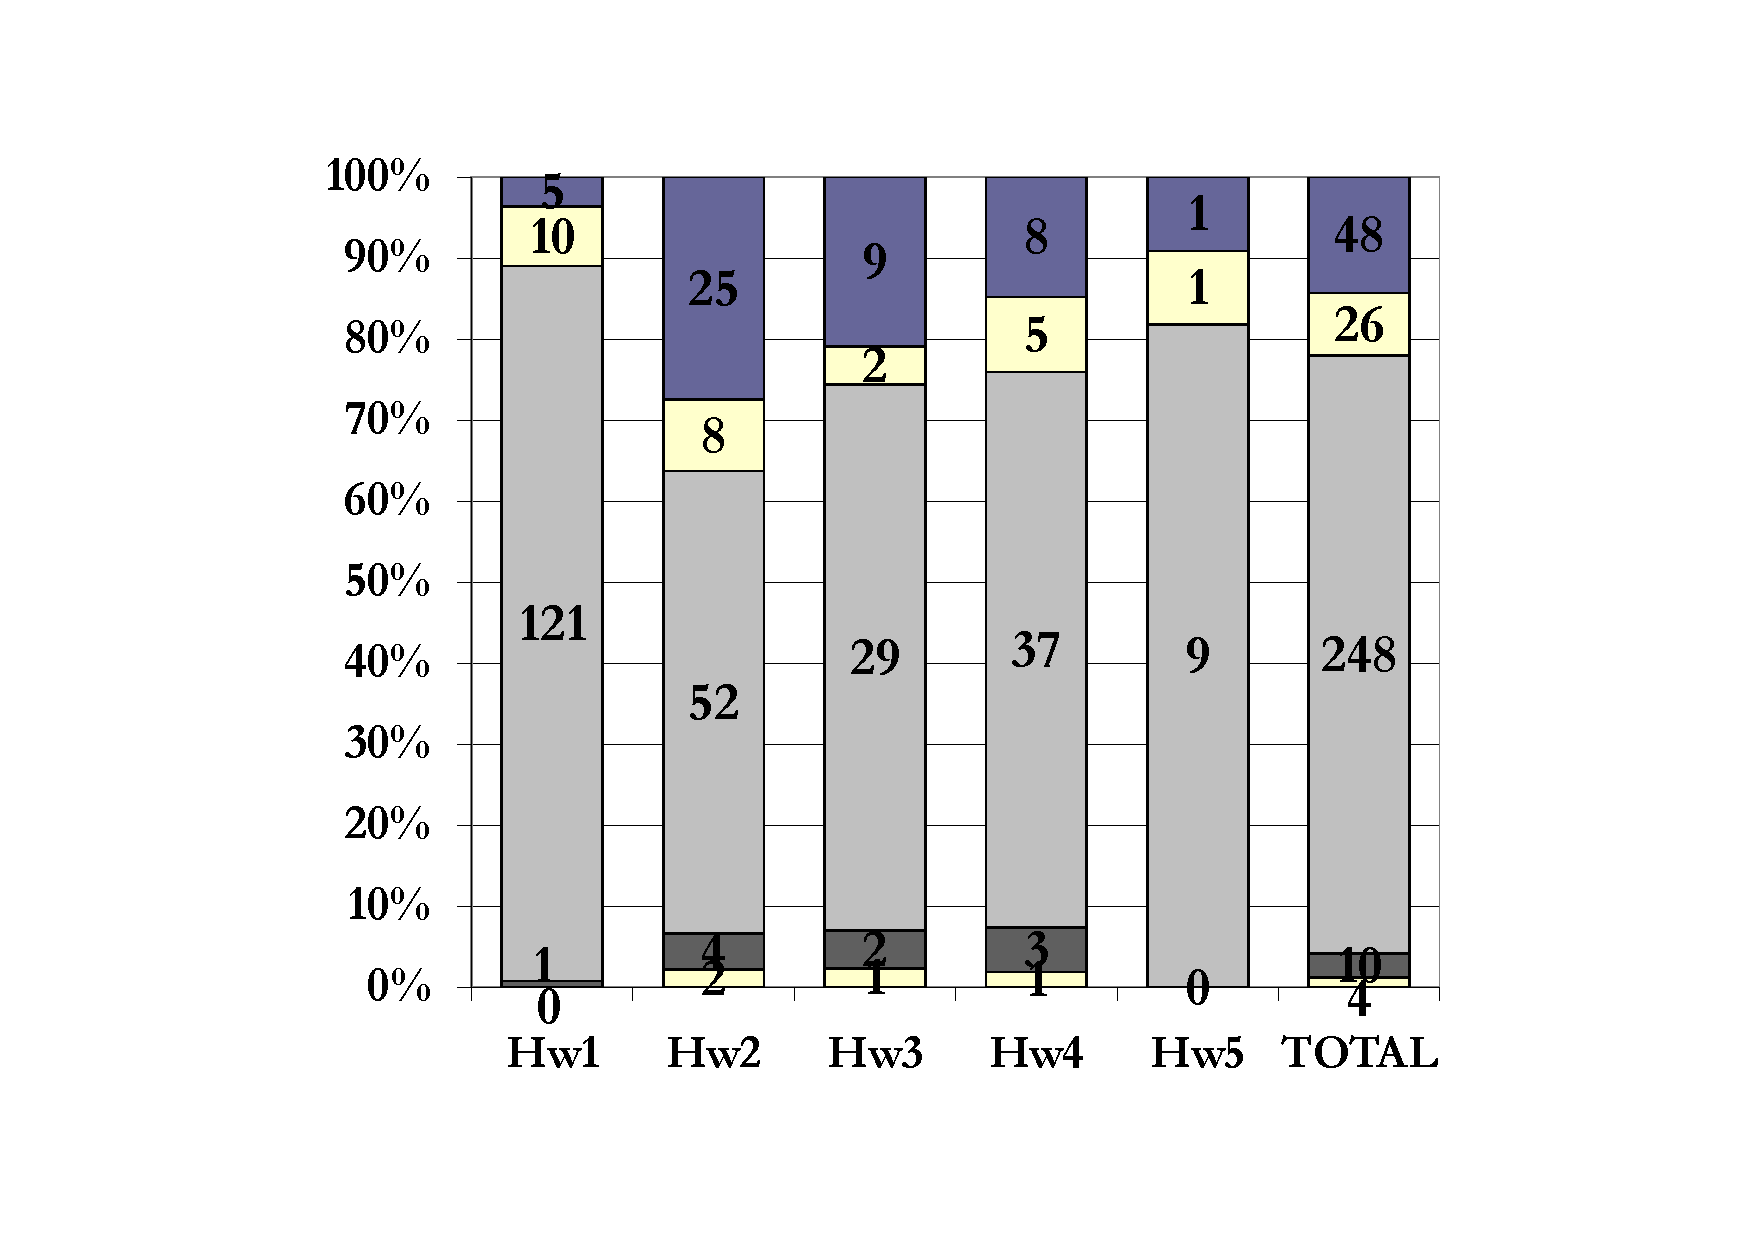
\includegraphics[height=16em]{graph/ocaml}
    \label{fig:consgraph:first}
}
%
\subfigure[Comparison with Seminal]{
    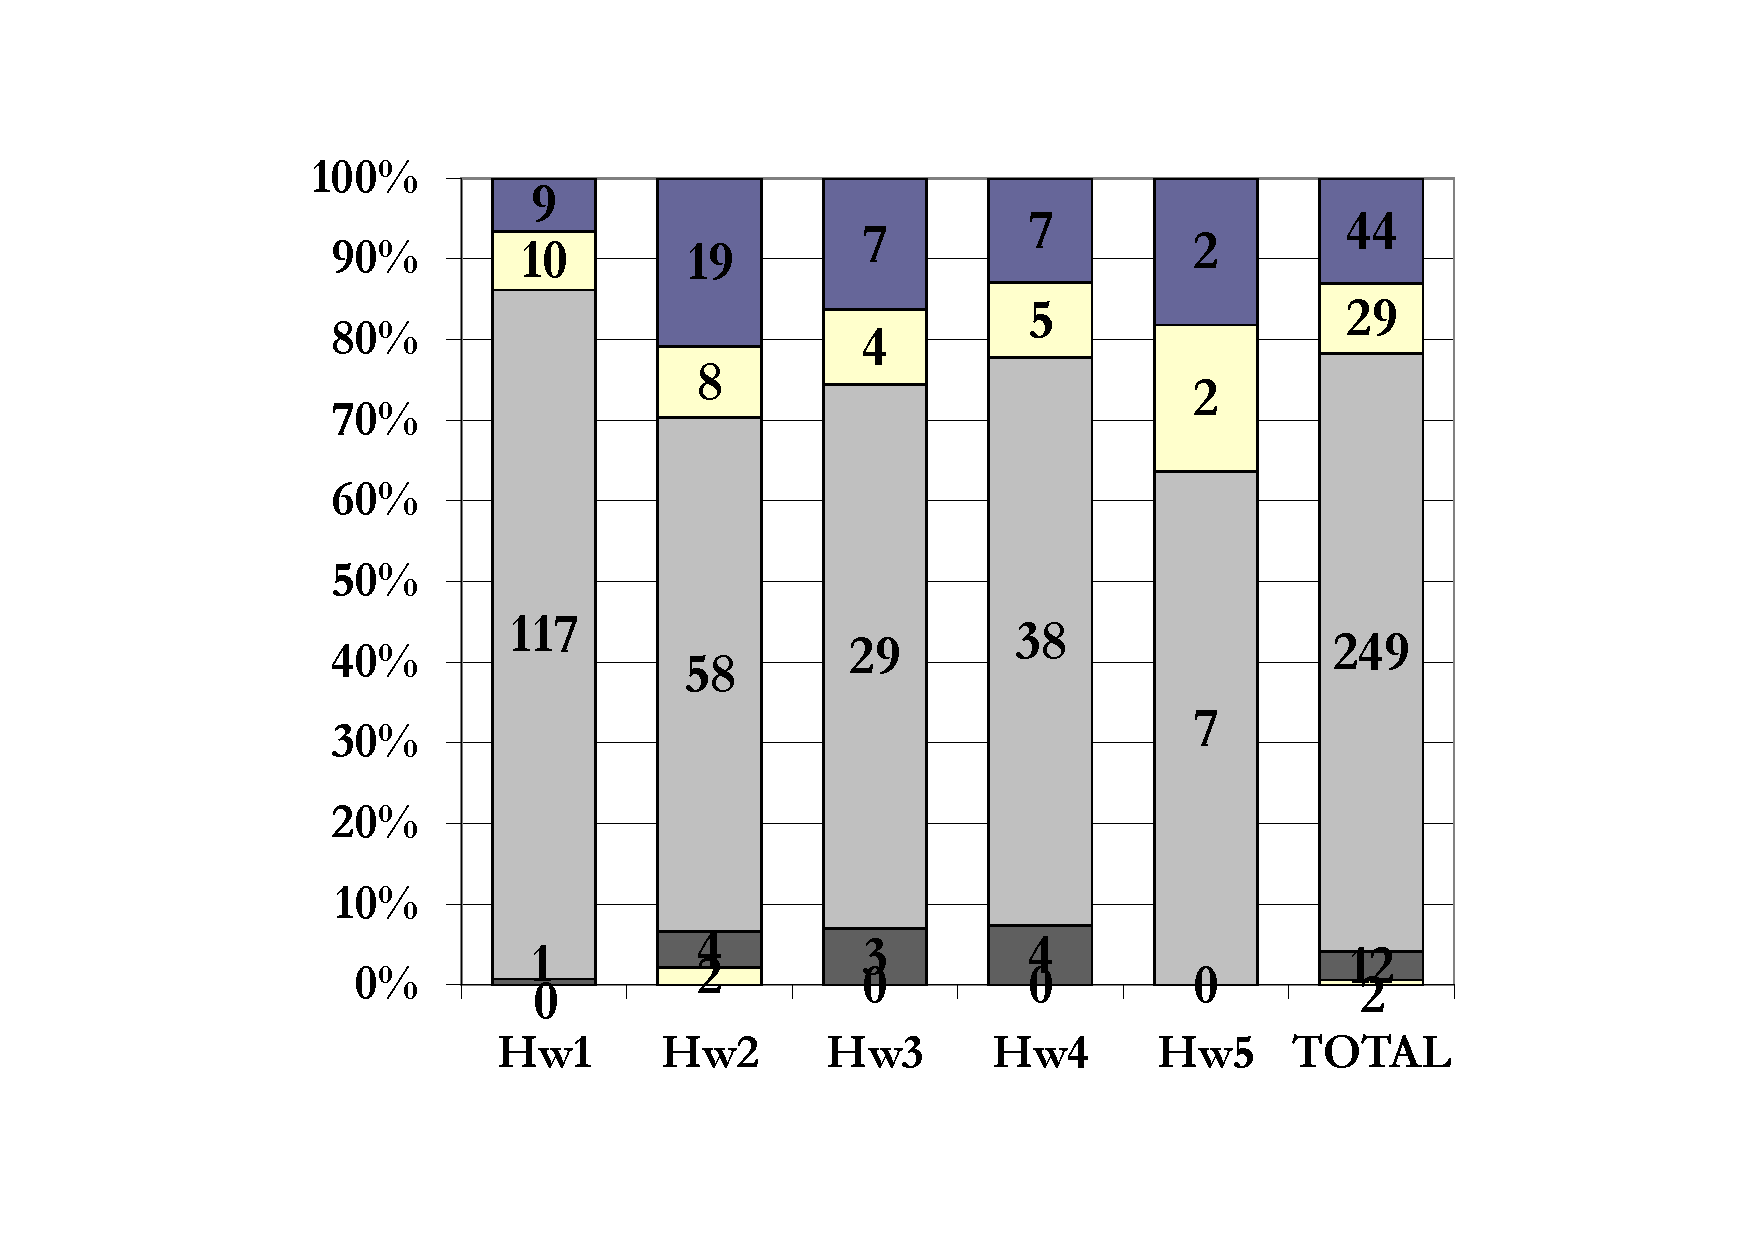
\includegraphics[height=16em]{graph/seminal}
    \label{fig:consgraph:second}
}
\end{center}
\caption{Results separated by student and by homework assignment.
Moving from bottom to top, the stacks represent OCaml programs where
%
(1) our tool miss the error location while the other tool identifies
one of them; 
%
(2) both approaches miss the error location; 
%
(3) both approaches report the correct error location; 
%
(4) both approaches report the correct error location, but our tool
reports multiple (correct) error locations; 
%
(5) our tool finds correct error location that the other tool misses} 
\label{fig:ocamlresult}
\end{figure*}

\begin{figure}
\begin{center}
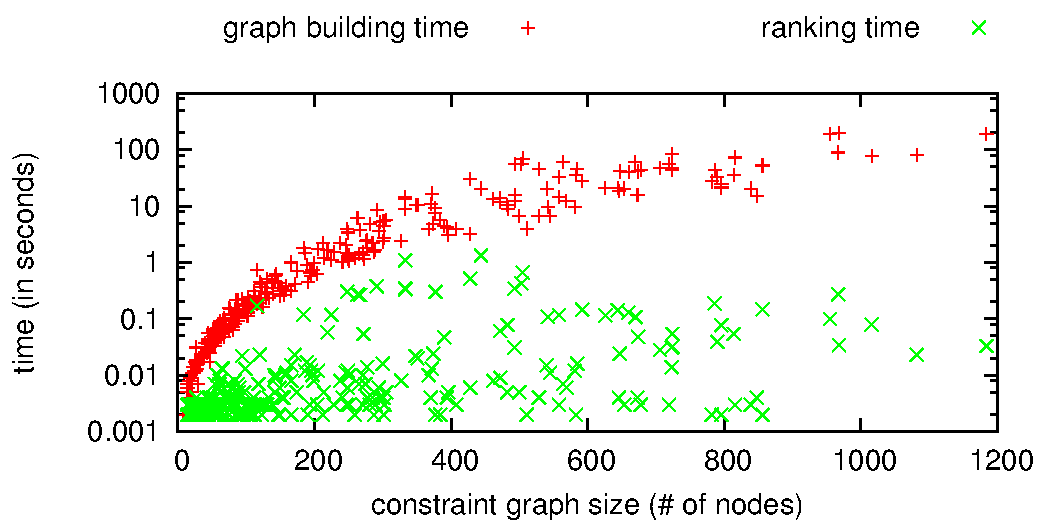
\includegraphics[height=14em]{graph/ocaml-performance}
\end{center}
\caption{Performance} 
\label{fig:performance}
\end{figure}

From the data, we analyze only type mismatch errors, which corresponds
to unsatisfiable constraints. Errors such as unbound values, too many
arguments to a constructor are usually better localized and they are
not the focus of our work. 

We also exclude programs using unsupported features of the modified
easyOCaml and files where the user's fix is unclear. After excluding
these files, there are 336 samples left.

For each file we analyze, we consider both the error location reported
by OCaml and the top rank suggestion of our tool. Since the Seminal
tool~\cite{lerner:pldi07} is not directly available, we reused the data
offered by the authors, who labeled the correctness of Seminal's error
location report.

We classify the files into one of the following five
categories and summarize the results in Figure~\ref{fig:ocamlresult}.

\begin{enumerate}
\item Our approach suggests error location that matches programmer's
fix, but the other tools' location missed the error.

\item Our approach reports multiple correct error locations that
matches programmer's fix, but the other tools' only reports one of
them.

\item Both approaches find the error locations corresponding to
programmer's fix.

\item Both approaches miss the error locations corresponding to
programmer's fix.

\item Our tool misses the error location but the other tool captures
it.
\end{enumerate}

The result shows that although OCaml's and Seminal's reports on error
locations differ across files, the overall quality is very similar:
they find around $80\%$ of the error locations correctly, but miss the
rest. 

Compared with both OCaml and Seminal, our tool consistently identifies
a higher percentage of error locations,
ranging from $93\%$ to $100\%$, with an average of $96\%$.

In about $7\%$ of
cases, our tool reports multiple error locations at once.
According to the data, the programmers typically fix these errors one
by one as the OCaml compiler only reports one at a time.
Reporting multiple errors at once may be more helpful.

\paragraph{Limitation of our approach}
Of course, our tool does miss errors. We studied
programs where our tool missed the error location, finding that
in each case it involved multiple interacting errors. In some cases
the programmer made a similar error multiple times.
the same way. Our tool fails to identify such errors because
it violates the assumption of error independence.
However, as our result suggests, this situation is rare.

The comparison between the tools is not completely apples-to-apples.
Recall that we only collect type mismatch errors in the evaluation.
OCaml is very effective in finding some localized program errors such as
unbound variables or wrong numbers of arguments; Seminal not only
finds errors but also proposes fixes, which our tool does not do.
%It can also identify some errors that are out of scope for our tool,
%such as swapped or missing arguments, error types we did not evaluated
%in this work.
In fact, these tools appear to be complementary.
%different kinds of errors. A combination of our tool and other
%technique is among our future work.

%Although our tool does have its limitations, it is more general
%than OCaml and Seminal are application specific, 

\subsubsection{Performance}

We measure the performance of
our tool on a Ubuntu 11.04 system using a dual core at 2.93GHz with 4G
memory. We separate the time spent on generating and inferring LEQ
edges in the graph and computing the rankings. Results are shown in
Figure~\ref{fig:performance}.

The results show that the running time of either graph building
time and ranking time scale with increasing constraint graph
size. One interesting observation is that the graph size has less
impact on the running time of our inference algorithm. We suspect the
reason is that the running time of our ranking algorithm is
dominated by the number of unsatisfiable paths identified in the graph,
which has a small correlation with graph size.

Considering graph construction time, over $99\%$ are done in 2
minutes.  Ranking is more efficient, where over $99\%$ can be done in
1 second.  Considering the human cost to identify error locations, the
performance seem acceptable.

\if 0
\begin{table}
\subfigure[Ranking time]{
\centering
\begin{tabular}{|c | c|}
\hline
Time & Percentage \\
\hline
0--0.01 & 74.20\% \\
\hline
0.01--0.1 & 17.20\% \\
\hline
0.1--1 & 7.96\% \\
\hline
1--10 & 0.64\% \\
\hline
Total & 100\% \\
\hline
\end{tabular}
\label{table:rankingtime}}
\subfigure[Graph construction time]{
\centering
\begin{tabular}{|c | c|}
\hline
Time & Percentage \\
\hline
0--0.01 & 7.89\% \\
\hline
0.01--0.1 & 29.97\% \\
\hline
0.1--1 & 23.97\% \\
\hline
1--10 & 19.56\% \\
\hline
10--100 & 17.67\% \\
\hline
$>100$ & 0.94\% \\
\hline
Total & 100\% \\
\hline
\end{tabular}
\label{table:graphtime}}
\caption{Performance results}
\end{table}
\fi

\subsection{Case study: Jif hypothesis inference}
\label{sec:jifeval}
We also evaluated how helpful our hypothesis inference algorithm is
for Jif. We have found missing hypotheses to be a common
source of errors in our experience with using Jif.

A corpus of buggy programs was harder to find for Jif than for OCaml.
We took 4 applications developed for other projects using either Jif
or Fabric (a Jif extension). These applications are interesting since
they deal with real-world security concerns.

To mimic the potential errors programmer would meet while writing the
application, we randomly remove hypotheses from these programs. In
total, we generate 40 files missing 1--5 hypotheses, the proportion of
each application approximately corresponds to the complexity of
application, measured by lines of code.

For all files we generated in this way, we classify each file into
one of four categories, with results summarized in
Table~\ref{table:hyporesult}.

\begin{enumerate}
\item The program passed Jif/Fabric label checking after removing the
hypotheses: the programmer made unneeded assumptions.

\item The generated missing hypotheses matches the one we remove.

\item The generated missing hypotheses provides a weaker assumption
that removes error, compared with the one we remove.

\item Our tool fails to find a suggestion better than the one
removed.
\end{enumerate}

The number of redundant assumptions in these
applications is considerable ($40\%$). We suspect the reason is that
the security model in these applications are nontrivial, so
programmers have difficulty formulating their security assumptions.
%They have to write down additional assumptions to pass the compiler.
This observation suggests that the ability to automatically infer
the missing hypothesis could be very useful to the programmers.

All the automatically inferred hypotheses had at least the same quality as
manually written ones.
%Although a more systematic way of
%evaluating real-world errors,
This preliminary result suggests that our hypothesis inference
algorithm is very effective and should be useful to programmers.
 
\section{Related Work}

\paragraph{Program analyses, constraints and graph} 

Modeling program analyses via constraint solving is not a new idea.
The most related work is set-based constraint program
analysis~\cite{aiken-setconstraint, aiken-typeinclusion}.  However,
these constraint languages do not model hypotheses, which is important
for some program analyses such as information-flow control.
 
Program slicing, shape analysis, and flow-insensitive points-to
analysis are amenable to graph-reachability~\cite{reps-graph}. Melski
and Reps~\cite{melski-cflgraph} show the interchangeability between
context-free-language reachability (CFG-reachability) and a subset of
set-based constraints. But only a small set of constraints---in fact,
a single variable---may appear on the right hand side of a partial
order. Moreover, no error diagnostic approach is proposed for the
graphs.

\paragraph{Error diagnoses for type inference
	    and information-flow control} 

Due to the unsatisfactory quality of error reports, a considerable
amount of work has been done on improving the error messages of both
ML-like languages and Jif.

Efforts on improving ML-like language type-error message can be
traced back to the early work of Wand~\cite{wand-errorfinding} and
of Johnson and Walz~\cite{johnson-popl86}. These two pieces of work
represent two directions in improving type-error messages: the former
traces _everything_ that contributes to the error, whereas the
latter attempts to infer the _most likely_ cause. We only discuss the
most related among them in this paper. More details can be found in
Heeren's summary~\cite{heeren:thesis}.

In the first direction, several efforts~\cite{choppella95,
haack:slicing, tip:slicing} improve the basic idea of
Wand~\cite{wand-errorfinding} in several ways. Despite the
attractiveness of feeding a full explanation to the programmer, the
reports are usually verbose and hard to follow.
\ACM{Can we cite anything for this claim of verbosity etc.? Right
now it is an unsupported assertion that doesn't sound very scientific.}

In the second direction, one approach is to alter the order of type
unification~\cite{lee:toplas, mcadam:unification}. However, since
error location may appear anywhere in the unification procedure, any
specific order fails in some circumstance. Some previous works tries
to advise the programmer how to fix the error.
McAdam~\cite{mcadam:thesis} suggests using morphisms along with
standard type inference to identify potential fixes for type errors.
Lerner et al.~\cite{lerner:pldi07} try to produce type-error messages
by trying changes to the AST until a program type-checks.  However,
both approaches are fairly specific to type inference. There is no
easy way to extending them to information-flow control analysis, for
instance.

For information-flow control, King et. al.~\cite{king:fse} propose to
generate a trace of information flow explaining the information-flow
violation in program. Despite the fact that this approach also
constructs a diagnosis from a dependency graph, only a subset of DLM
model is handled. In particular, hypotheses are not supported.
Moreover, as in type-error slicing, reporting a whole path can be
too verbose for the programmer.  Merlin~\cite{livshits:merlin} uses
probabilistic inference to automatically infer explicit information
flow specifications from program code; this is a different
application from our paper.\ACM{maybe we can say more about why Merlin
is relevant.}

\paragraph{Missing hypothesis inference}

The most related work on inferring likely missing hypotheses is the
recent work on error diagnosis using abductive
inference~\cite{dillig:pldi12}. This work computes small, relevant
queries presented to a user that capture exactly the information a
program analysis is missing to either discharge or validate the error.
It handles first-order logic, but there is no straightforward
way to encode our constraint language into first-order logic.
Also, our missing-hypothesis inference is more straightforward.
\ACM{Is it less powerful, though? Sounds a bit subjective.}

% Automatic instrumentation~\cite{king:esop10}
% Policy inference~\cite{chong:sp11, harris:ccs10}.
% Using statisctical
% analysis for bug finding is not new. Dawson Engler.

\section{Conclusion}

Better tools for helping programmers find the errors resulting from
program analysis will make programmers more willing to use the many
powerful program analyses that have been developed. This paper has
introduced an analysis of program constraint graphs that offers a
powerful and general way to diagnose both locations of errors in
programs and missing environmental hypotheses.

The results using our tool with relatively little OCaml-specific or
Jif-specific customization suggest it is a promising approach for
diagnosing program analysis errors.

There are clearly many interesting directions to take this work.
Though we have shown that the technique works well on two very
different type systems, it would likely be fruitful to apply these
ideas to other type systems and program analyses, and to explore more
sophisticated ways to estimate the likelihood of different error
explanations.

\bibliographystyle{abbrv}
\bibliography{constraint,../bibtex/pm-master}

\end{document}
